
\section{INTRODUCTION}
\subsection{Fractional Derivatives}
\begin{frame}{INTRODUCTION}
\framesubtitle{Fractional Derivatives}
\begin{multicols}{2}
    \textbf{Pros}
    \begin{itemize}
        \item Generalization of ordinary derivatives.
        \item Nonlocal operators $\longrightarrow$ Memory and heritage.
        \item More accuracy and robustness.
        \item Unexplored areas and applications.
    \end{itemize}
    \columnbreak
    \textbf{Cons}
    \begin{itemize}
        \item There are multiple fractional derivatives definitions.
        \item The derivatives are not always in terms of elementary functions.
        \item Some definitions require strong conditions on the functions to differentiate.
    \end{itemize}
    \end{multicols}
\end{frame}

\subsection{Caputo Definition}
\begin{frame}{INTRODUCTION}
\framesubtitle{Caputo Definition}
The Caputo definition of fractional derivative is
\begin{equation}
    \mathcal{D}_C^\alpha y(t) = J^{m-\alpha}y^{(m)}(t) = \dfrac{1}{\Gamma(m-\alpha)}\int_0^t \dfrac{y^{(m)}(\lambda)}{(t-\lambda)^{1-m+\alpha}}d\lambda
\end{equation}
where $\alpha\geq0$, $m=\ceil{\alpha}$, $\Gamma(\cdot)$ is the gamma function and $J^{m-\alpha}$ is the Riemann-Liouville integral. From now on, the Caputo-type fractional derivative will be denoted as
\begin{equation}
    \mathcal{D}_C^\alpha y(t)=\dfrac{d^\alpha}{dt^\alpha}y(t)
\end{equation}
For example
    \begin{align*}
        \dfrac{d^{0.5}}{dt^{0.5}} [t]&= \dfrac{1}{\Gamma(1-0.5)}\int_0^t \dfrac{d}{d\lambda}(\lambda)\cdot\dfrac{d\lambda}{(t-\lambda)^{1-0.5+1}}\\
      &= \dfrac{1}{\sqrt{\pi}}\int_0^t \dfrac{d\lambda}{(t-\lambda)^{1/2}}\quad\text{, let $u=t-\lambda$ $\rightarrow$ $du=-d\lambda$.}\\
      &= \dfrac{1}{\sqrt{\pi}}\int_0^t \dfrac{du}{u^{1/2}}\\
      &=2\sqrt{\dfrac{t}{\pi}}
    \end{align*}
\end{frame}

\subsection{Riemann-Liouville Integral}
\begin{frame}{INTRODUCTION}
\framesubtitle{Riemann-Liouville Integral}
The Riemann-Liouville integral of order $\alpha$ is defined as
\begin{equation}
    J^\alpha y(t) = \dfrac{1}{\Gamma(\alpha)}\int_{0}^{t}\dfrac{y(\lambda)}{(t-\lambda)^{1-\alpha}}d\lambda
\end{equation}
\textbf{Properties}\\\vspace{0.5cm}
\begin{itemize}
    \item
    \begin{equation}
        J^{\alpha}\left[f(t)+g(t)\right]=J^\alpha f(t)+J^\alpha g(t)
    \end{equation}
    \item \begin{equation}
        J^\alpha J^\beta f(t) = J^{\alpha+\beta} f(t)
    \end{equation}
    \item \begin{equation}
        \dfrac{d^\alpha}{dt^\alpha}\left[ J^\alpha y(t)\right] = y(t)
    \end{equation}
    \item \begin{equation}
            J^\alpha \left[ \dfrac{d^\alpha}{dt^\alpha}y(t)\right] = y(t) - \sum_{r=0}^{m-1}\dfrac{y_rt^r}{r!}
        \end{equation}
\end{itemize}
\end{frame}


\subsection{The Tautochrone Problem}
\begin{frame}{INTRODUCTION}
    \framesubtitle{The Tautochrone Problem}
    It is desired to find a curve such that, if an object starts on any point along this curve, the time that it requires to slide down to the origin is the same.
    
    \begin{multicols}{2}
    \begin{itemize}
        \item Tauto $\rightarrow$ equal.
        \item Chrono $\rightarrow$ time.
        \item Abel, XVIII century.
    \end{itemize}
    Assumptions:
    \begin{itemize}
        \item The object moves only by the force of gravity.
        \item It moves without friction.
    \end{itemize}
    \columnbreak
    \begin{figure}[H]
        \centering
        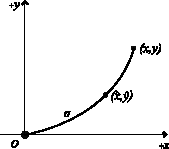
\includegraphics[scale=1.25]{files/taut.pdf}
        \caption{Tautochrone problem.}
    \end{figure}
    
    \end{multicols}
    \begin{center}
    \href{run:gify.gif}{Click for GIF}
    \end{center}
    
\end{frame}


\begin{frame}{INTRODUCTION}
\begin{multicols}{2}
    \framesubtitle{The Tautochrone Problem}
    Using the energy conservation law,
    \begin{align*}
         mgy =& \dfrac{1}{2}m\left(\dfrac{d\sigma}{dt}\right)^2 + mg\hat{y}\\
         \vdots\\
        \dfrac{d^{0.5}}{dy^{0.5}} \sigma ( y ) &= \frac { \sqrt { 2 g } } { \Gamma \left( \frac { 1 } { 2 } \right) } T
    \end{align*}
    Through some analytical procedures, we obtain
    \begin{align*}
        x &= \dfrac{gT^2}{\pi^2}[t+\sin(t)]\\
        y &= \dfrac{gT^2}{\pi^2}[1-\cos(t)]
    \end{align*}
    
    \columnbreak
    \begin{figure}[H]
        \centering
        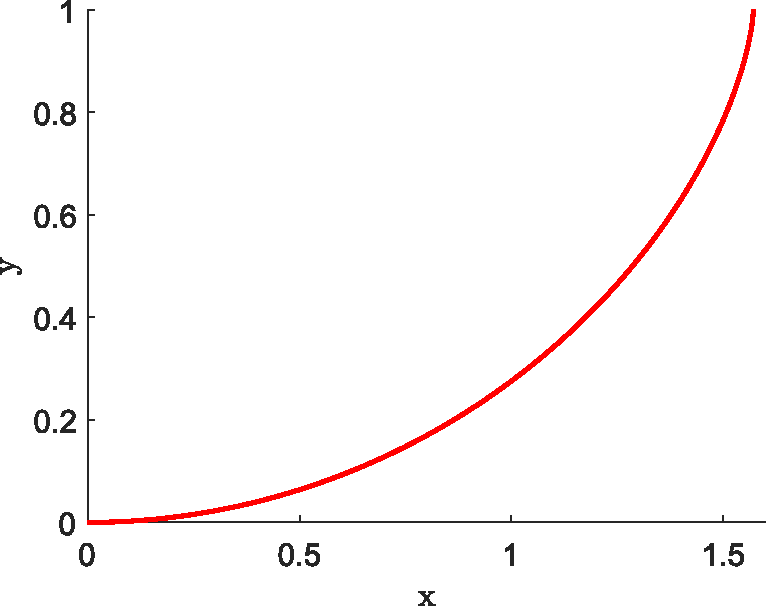
\includegraphics[scale=0.4]{files/tautochrone.pdf}
        \caption{Tautochrone curve.}
        \label{fig:my_label}
    \end{figure}
    \end{multicols}
\end{frame}